\documentclass{beamer}
\usetheme{Madrid}
\title{Visualisierung eines schiefen Wurfs in C++}
\author{Mert Düzgün \and Gianluca Fuwa}

\begin{document}
\begin{frame}
  \titlepage
\end{frame}
\begin{frame}
\tableofcontents
\end{frame}

\section{Zielsetzung des Programms}
\begin{frame}
\begin{itemize}
\item Visualisierung des schiefen Wurfs mittels GUI
\item Plot der Höhe des Wurfes zur Wurfdauer
\item Anfangsgeschwindigkeit, Wurfwinkel und Anfangshöhe
als Eingabewerte 
\end{itemize}
\end{frame}

\section{Visualisierung mittels FLTK}
\subsection{FLTK als GUI}

\begin{frame}{Voraussetzungen}
  \begin{itemize}
  \item {dynamic memory allocation} 
  \item new ... belegt dynamischen Speicherplatz
  \item { a -\textgreater x:=(*a).x
  \end{itemize}
\end{frame}

\begin{frame}{zu FLTK Klassen}
\begin{itemize}
\item Shape und Vererbungen
\item Widget und Vererbungen
\item Window 
\item attach-Funktionen virtual
\item draw-Funktionen virtual
\end{itemize}
\end{frame}

\subsection{Klassen zur Programmierung mit FLTK}
\begin{frame}{Shape}
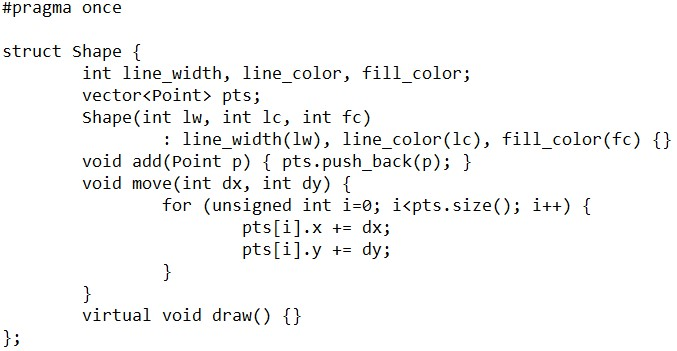
\includegraphics[scale=0.63]{FLTK_Shape.jpg} 
\end{frame}

\begin{frame}{FLTK Window}
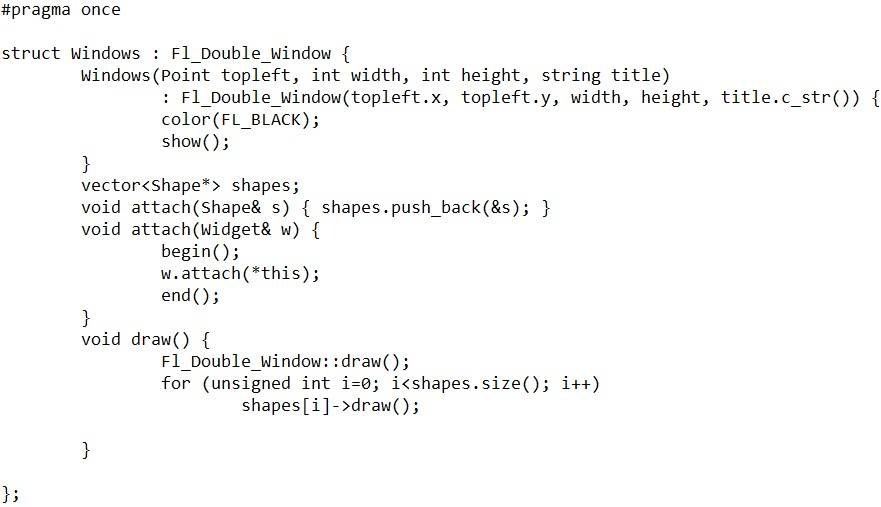
\includegraphics[scale=0.63]{FLTK_window.jpg} 
\end{frame}

\begin{frame}{Text}
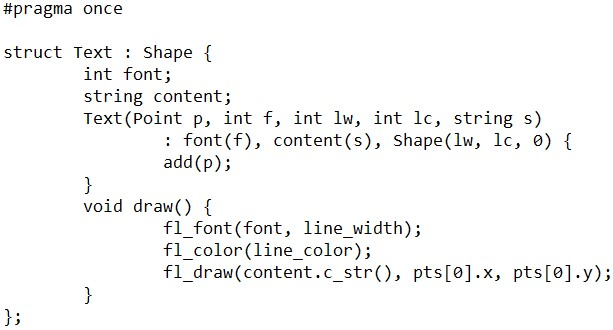
\includegraphics[scale=0.63]{FLTK_text.jpg}  
\end{frame}

\begin{frame}{Line}
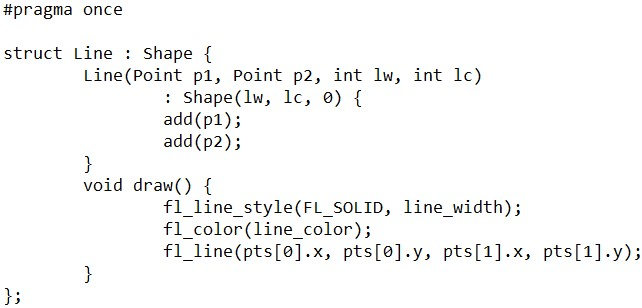
\includegraphics[scale=0.63]{../Pictures/FLTK_Line.jpg} 
\end{frame}

\begin{frame}{Circle}
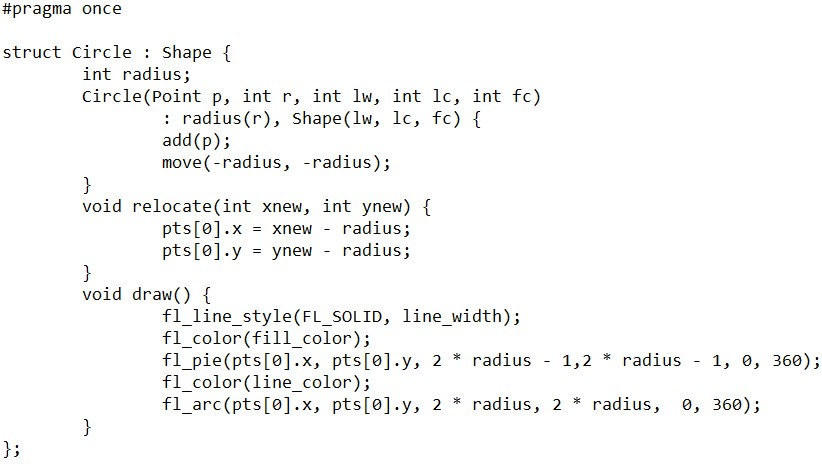
\includegraphics[scale=0.63]{FLTK_Circle.jpg} 
\end{frame}

\begin{frame}{Widgets in FLTK}
\begin{itemize}
\item Konstruiert mit Parametern x, y, w, h, label, cb
\item spezifische Unterklassen können Eingabewerte aufnehmen
\item Eingabewerte können in callback-Funktionen aufgerufen werden
\end{itemize}
\end{frame}

\begin{frame}{Widget}
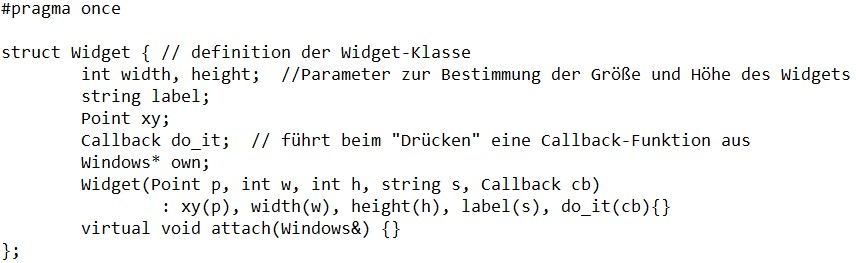
\includegraphics[scale=0.63]{FLTK_Widget.jpg} 
\end{frame}

\begin{frame}{FLTK Button}
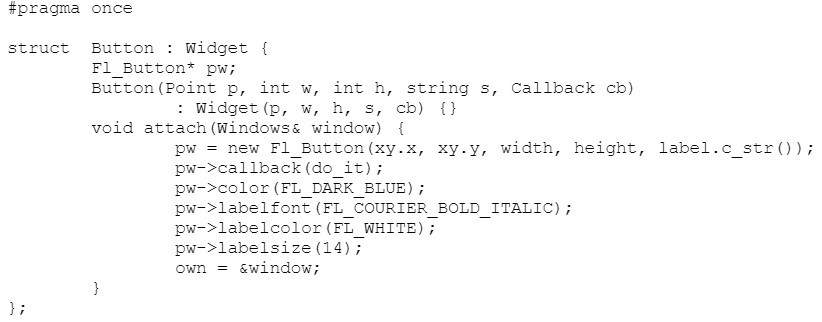
\includegraphics[scale=0.63]{FLTK_Button.jpg} 
\end{frame}

\begin{frame}{FLTK In Box}
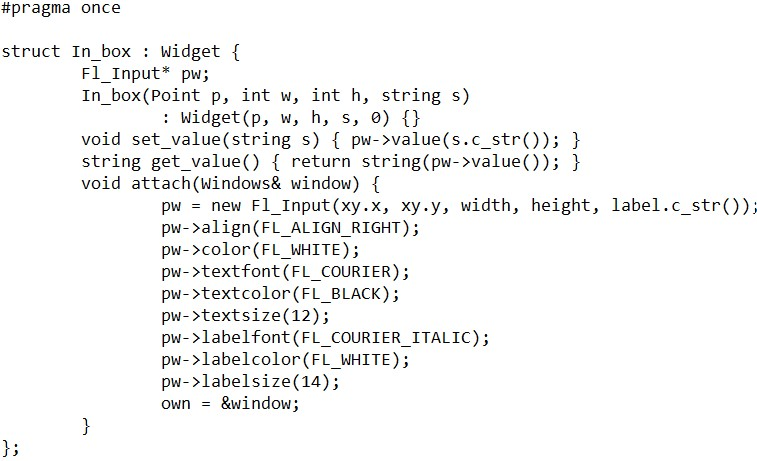
\includegraphics[scale=0.63]{In_Box.jpg} 
\end{frame}

\begin{frame}{FLTK Out Box}
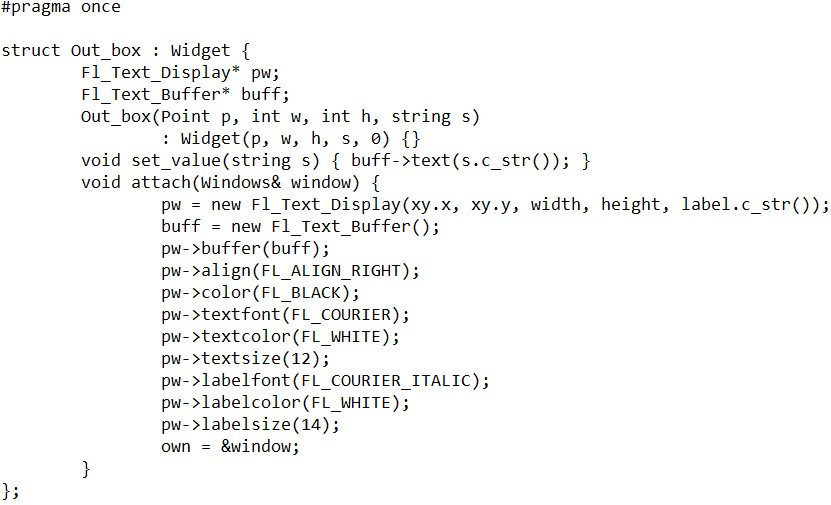
\includegraphics[scale=0.63]{Out_Box.jpg} 
\end{frame}

\begin{frame}{FLTK Slider}
\begin{itemize}
\item Schieberegler für die Ausgangshöhe
\item Widget-Unterklasse
\end{itemize}
\end{frame}

\begin{frame}{FLTK Slider}
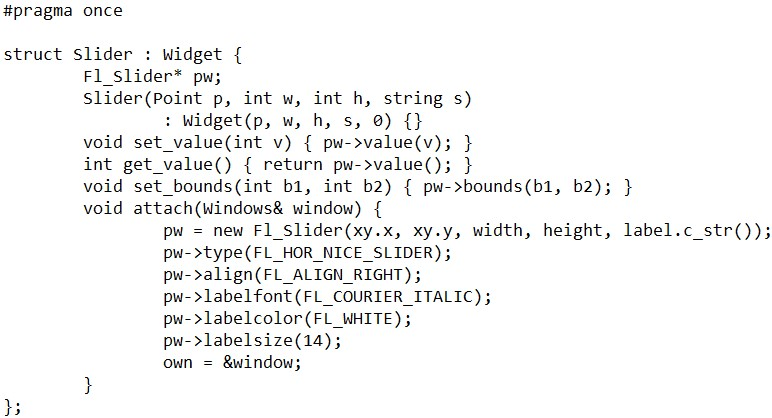
\includegraphics[scale=0.63]{Slider.jpg} 
\end{frame}

\begin{frame}{GUI Libraries}
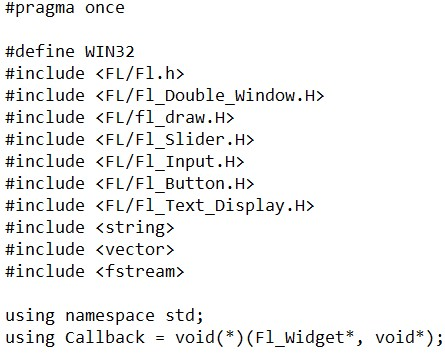
\includegraphics[scale=0.63]{GUITeil1.jpg} 
\end{frame}

\begin{frame}{GUI Libraries}
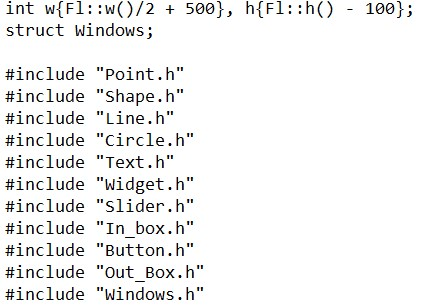
\includegraphics[scale=0.63]{GUITeil2.jpg} 
\end{frame}

\section{Callback-Funktionen}
\begin{frame}{Callback-Funktion}
\begin{itemize}
\item Callback-Funktionen von Widgets initialisiert
\item Parameter können von Widgets in die Funktion übergeben werden
\item get\textunderscore value
\item push\textunderscore back
\item Stoppuhr mit Chrono
\end{itemize}
\end{frame}

\subsection{Callback-Funktion 1}
\begin{frame}{Callback1}
\begin{itemize}
\item Ziel der Callback1-Funktion ist die Simulation des
Wurfes mit Stößen am Rand des Fensters
\item Geschwindigkeitsvektor wird definiert
\item Kreis wird bewegt und relocatet
\end{itemize}
\end{frame}
\begin{frame}{Callback1}
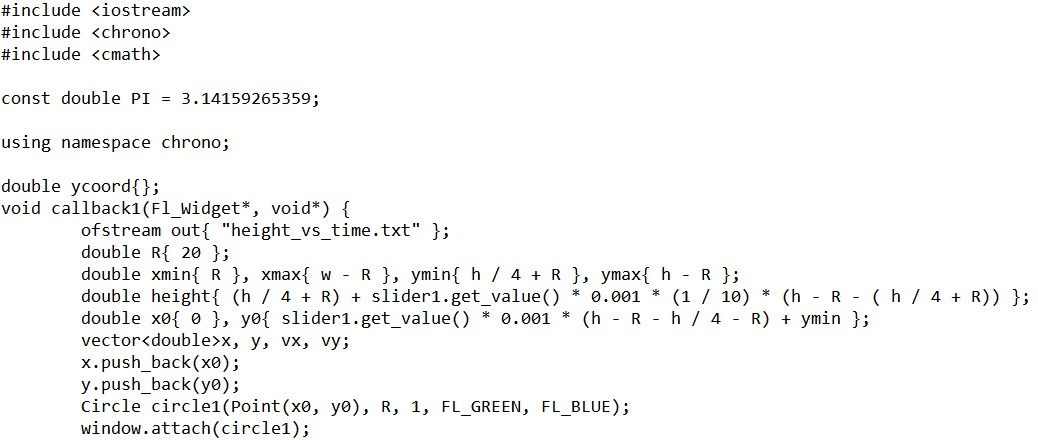
\includegraphics[scale=0.5]{Callback1Teil1.jpg} 
\end{frame}

\begin{frame}{Callback1}
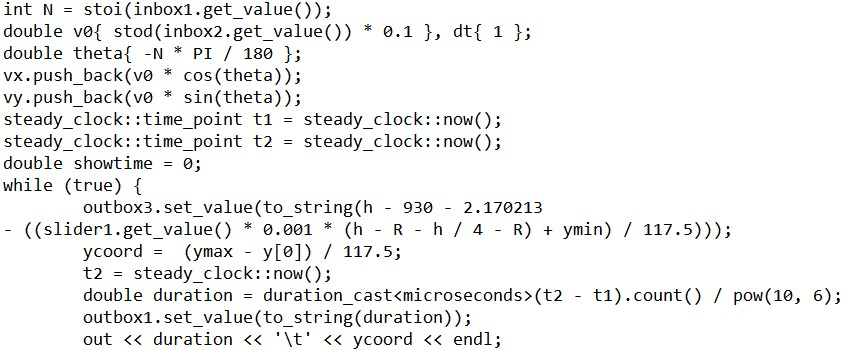
\includegraphics[scale=0.63]{Callback1Teil2.jpg} 
\end{frame}

\begin{frame}{Callback1}
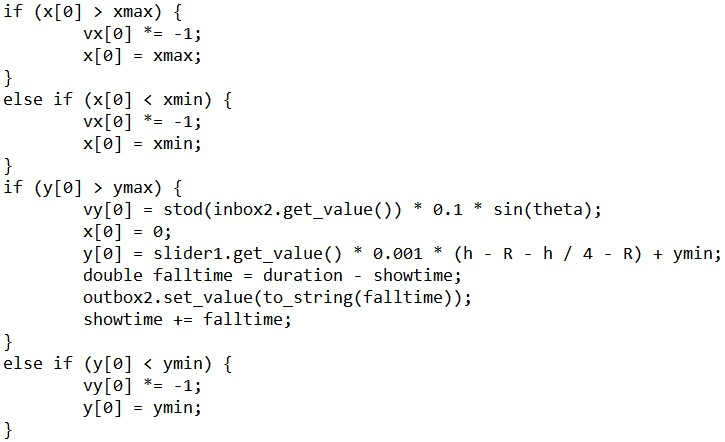
\includegraphics[scale=0.6]{Callback1Teil3.jpg} 
\end{frame}

\begin{frame}{Callback1}
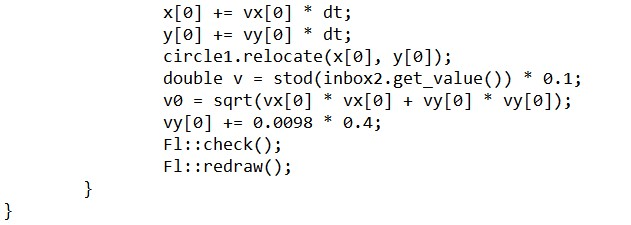
\includegraphics[scale=0.63]{Callback1Teil4.jpg} 
\end{frame}

\subsection{Callback-Funktion 2}
\begin{frame}{Callback2}
\begin{itemize}
\item die in Callback1 gebildete Datei soll geplottet werden
\item Callback 2 soll die Daten mithilfe von gnuplot auswerten
\end{itemize}
\end{frame}

\begin{frame}{Callback2}
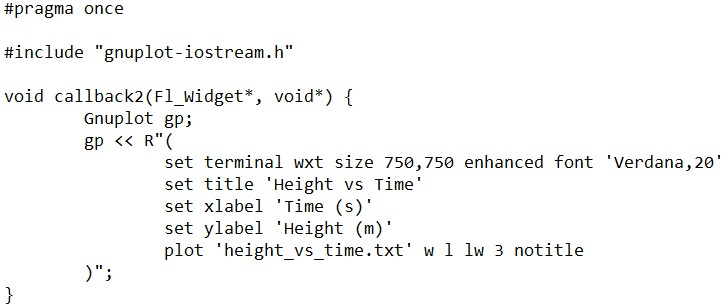
\includegraphics[scale=0.63]{Callback2.jpg} 
\end{frame}

\begin{frame}
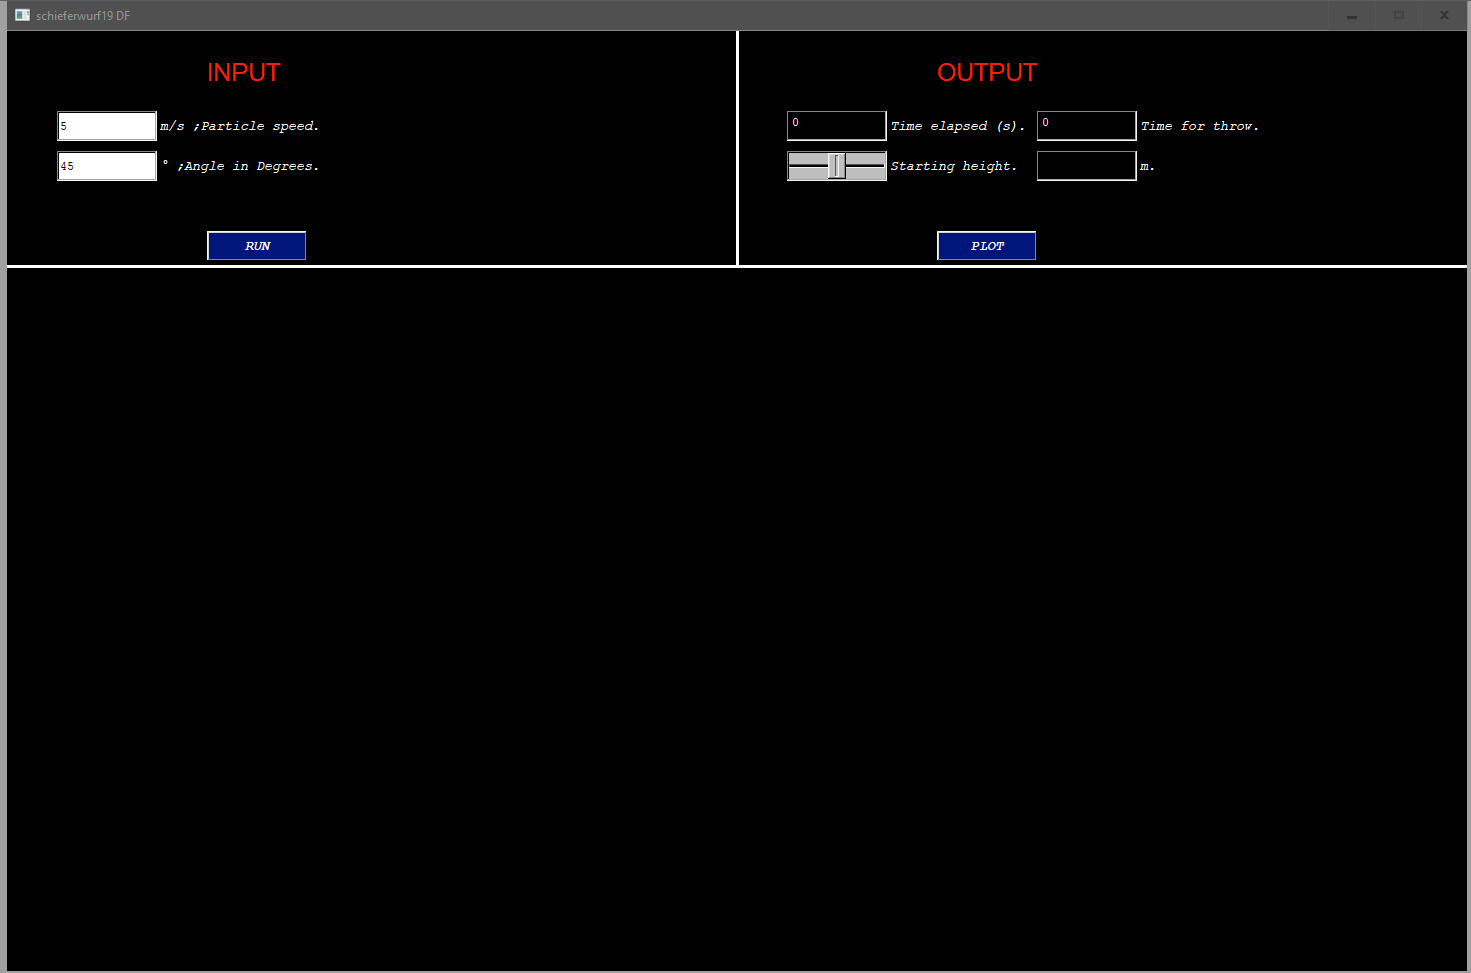
\includegraphics[scale=0.22]{IMG-20190705-WA0002.jpg} 
\end{frame}

\begin{frame}
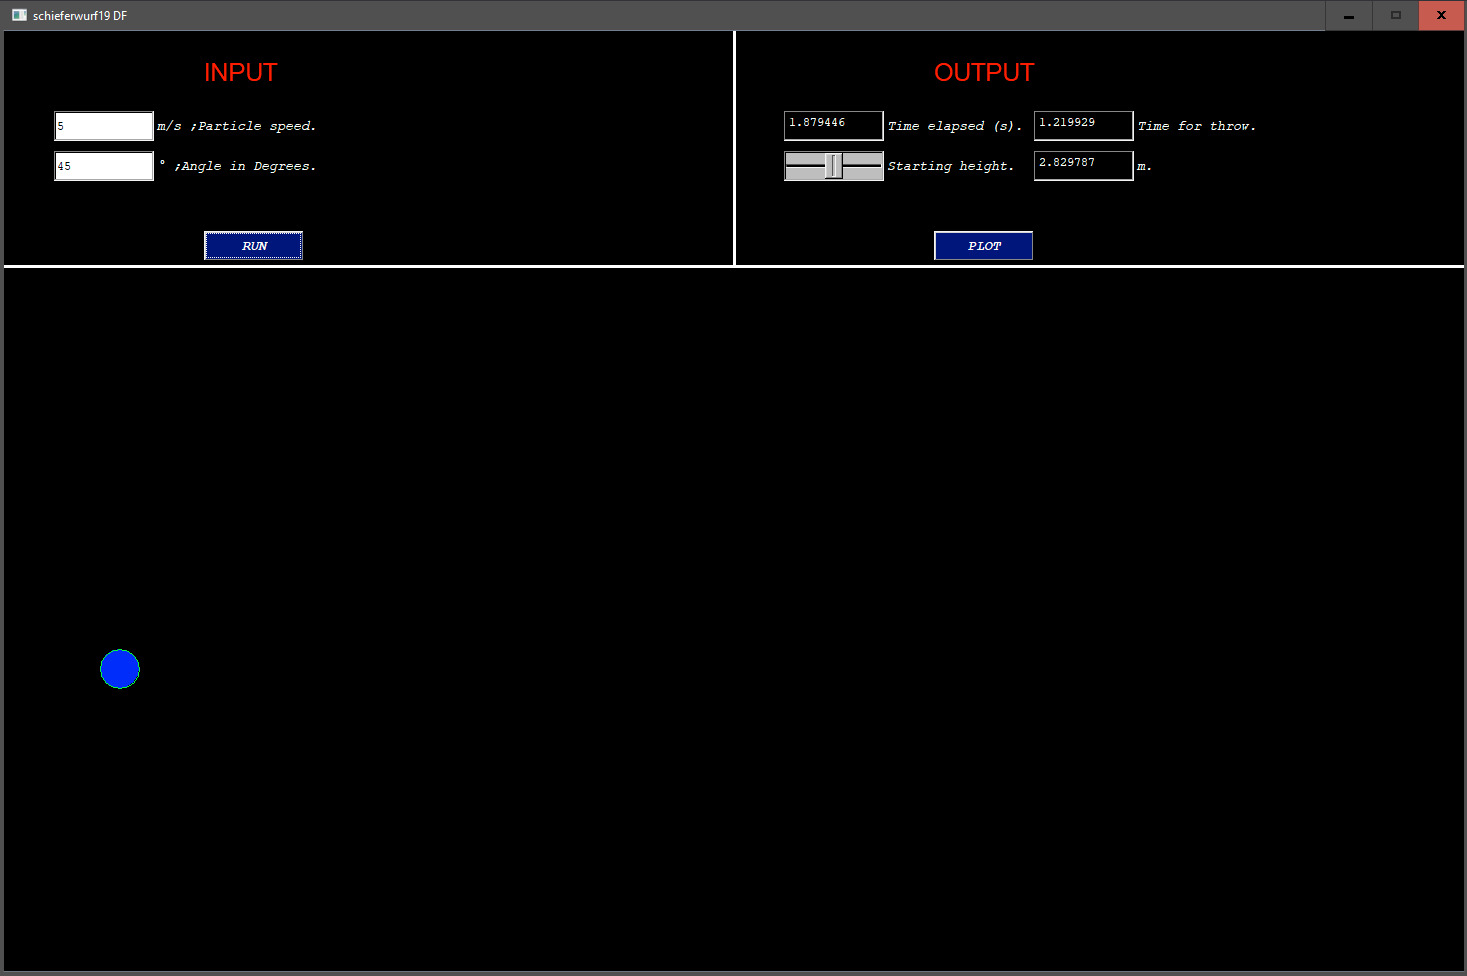
\includegraphics[scale=0.22]{IMG-20190705-WA0001.jpg} 
\end{frame}

\begin{frame}
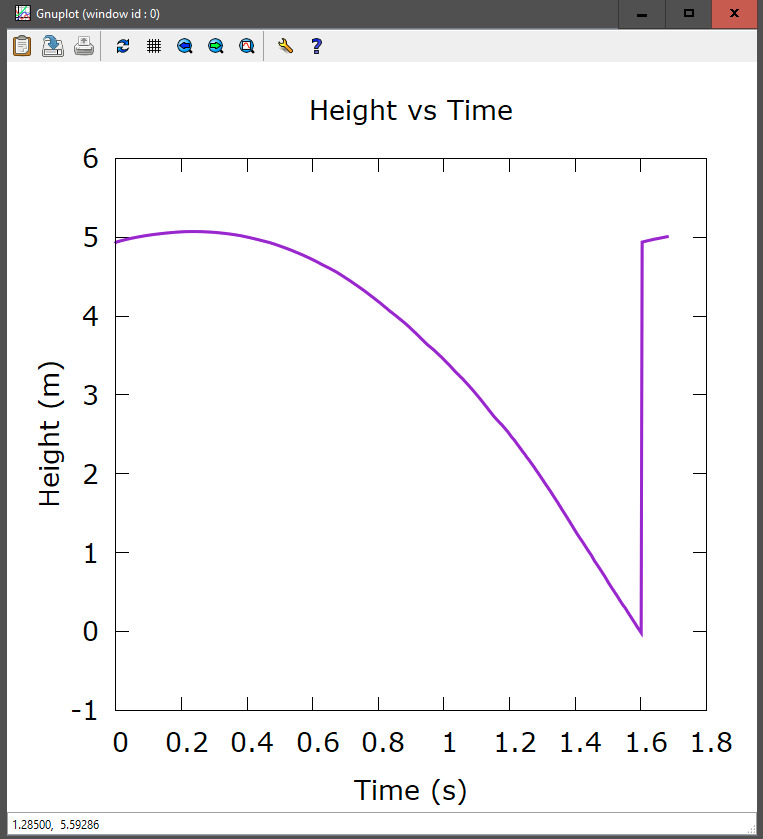
\includegraphics[scale=0.22]{IMG-20190705-WA0000.jpg} 
\end{frame}
\end{document}
